% 第 40 章　相对论的能量与动量
\chapter{相对论的能量与动量}

第 38 章和第 39 章改写了我们对时间和长度的认识：运动着的钟走得慢，运动着的尺缩得短，两件事是否“同时”发生取决于观察者。这一章要处理一件更实在的事情——能量和动量。它们是我们从力学一路用到电磁学、热力学的“记账本”，而相对论要告诉我们：这本账的记法也得改。改完之后，“质量”这个词将获得一个全新的、足以解释太阳为什么发光的含义。

\step{反常识开场}

\begin{mainline}
在瑞士和法国边境的地下，有一台周长约 27 千米的环形机器，叫大型强子对撞机。它用几千块超导磁铁推着质子一圈一圈地跑，每跑一圈，质子就从电场那里领到一份能量。工程师想让它领多少，它就能领多少——只要电费付得起。按理说，能量越领越多，速度就该越跑越快。可是测量结果像撞上了一堵看不见的墙：当质子的能量从 4500 亿电子伏特加到 65000 亿电子伏特，能量翻了十几倍，速度却几乎原地不动——它已经达到光速的 99.999999\%，再把能量翻一倍，速度与光速的差距只从每秒约 3 米缩小到每秒约 0.75 米。油门踩得动，速度表却不走了。这台全世界最贵的机器仿佛在抗议：你加的不是速度。

同一个谜题还有一个更古老的版本。太阳每秒向太空倾泻约 \(3.8\times10^{26}\) 焦耳的能量。假如太阳是一整颗煤球，就算它全是上等煤，又能烧多久？太阳的质量约 \(2\times10^{30}\) 千克，煤的热值约每千克 \(3\times10^{7}\) 焦耳，全部烧完释放约 \(6\times10^{37}\) 焦耳，按目前的亮度只够烧五千年上下——还不够人类文明史的长度。19 世纪的物理学家开尔文想得更细：太阳也许靠缓慢收缩、把引力能变成热来发光。可这样算，寿命也只有几千万年。与此同时，地质学家从岩层里读出地球的年龄是几十亿年。一边是物理学家的账，一边是石头里的证据，两边对不上。太阳到底在烧什么？

其实工程界早就撞过这堵墙，只是当时没人认得它。1930 年代，劳伦斯发明回旋加速器，原理是让带电粒子在磁场里兜圈，每半圈被电场推一把。这套设计依赖一个漂亮的巧合：按牛顿力学，粒子兜一圈的时间与速度无关，所以电场的节奏可以一劳永逸地定死。可当质子被加速到约两千万电子伏特以上，实验人员发现粒子渐渐跟不上电场的节拍，能量再也加不上去。机器没坏，是假设错了——粒子兜圈的时间悄悄变长了。事后用本章的语言看，原因一清二楚：粒子的动量是 \(\gamma mv\) 而不是 \(mv\)，多出来的那个 \(\gamma\) 改写了兜圈的节奏。工程师们没有放弃，他们让电场频率跟着粒子一起变慢，造出了“同步回旋加速器”，继续把能量往上推了一个量级。这是人类第一次不是在书本上、而是在机器的脾气里遇见相对论。

加速器里“加不动的速度”和太阳里“烧不完的燃料”，看似毫不相干，其实是同一条新规律的两张面孔。这条规律，就是本章要讲的相对论能量与动量。
\end{mainline}

\step{先猜一猜}

\begin{mainline}
在往下看之前，先把你自己的直觉摆到桌面上。下面四个说法，凭第一感觉判断哪些对、哪些错：

第一，加速器只要再多花一倍的电费，质子总有一天能超过光速。

第二，太阳内部一定藏着某种“超级燃料”，一克顶得上成百上千吨煤。

第三，两艘飞船各以四分之三倍光速相向飞行，从其中一艘看另一艘，相对速度是一点五倍光速——速度直接相加就行了。

第四，一个东西静止不动时，它身上谈不上有什么“能量”；能量是运动才有的属性。

请把你的答案写下来。读完本章再回头对照：你会发现第二条方向对了，但真相远比“超级燃料”奇怪——太阳烧的不是任何化学物质，它烧的是质量本身；而第四条错得最彻底，静止的东西身上恰恰藏着最大的一笔能量。
\end{mainline}

\step{动手实验}

\begin{experiment}[用计算器把一辆车推向光速]
你不需要粒子加速器，一台能开平方的计算器（手机就行）就能重现那堵“看不见的墙”。

设想一辆小车，它的“静能量”记为一份，写作 \(mc^{2}\)。现在规定一个游戏规则：每按一次按钮，你就给小车增加一份动量，大小恰好是 \(pc=mc^{2}\)，也就是让“动量乘光速”这个量一份一份地涨：1 份、2 份、3 份……

先用牛顿的老规则算速度：\(v/c=pc/(mc^{2})\)。按下去：1 倍光速、2 倍光速、3 倍光速——轻松突破光速，毫无阻碍。

再用本章要讲的相对论规则算：\(v/c=pc/E\)，其中 \(E=\sqrt{(pc)^{2}+(mc^{2})^{2}}\)。逐次按计算器：

动量 1 份：\(v/c=1/\sqrt{2}\approx0.71\)；

动量 2 份：\(v/c=2/\sqrt{5}\approx0.89\)；

动量 3 份：\(v/c=3/\sqrt{10}\approx0.95\)；

动量 10 份：\(v/c=10/\sqrt{101}\approx0.995\)；

动量 100 份：\(v/c\approx0.99995\)。

看出规律了吗？动量可以一份一份无限加下去，速度却像被光速这块磁铁吸住，永远停在一步之外。原因在于那个平方根：分母 \(E\) 总比分子 \(pc\) 多出 \((mc^{2})^{2}\) 这一项，所以 \(v/c\) 永远小于 1。你刚才只用到四则运算和开平方，就亲手重演了大型对撞机里真实发生的事情。
\end{experiment}

\begin{mainline}
还有一个不用任何仪器的“实验”，可以在厨房里做。拿两团一样大的橡皮泥，让它们相向滚动、迎面相撞，粘成一坨停在那里。撞之前两团都在动，都有动能；撞之后那坨泥静止不动，动能去哪了？伸手摸一摸：泥变温了。动能变成了热。这很平常。但请把这个问题留到本章后面：那坨粘住的泥，和原来两团泥相比，重量严格相等吗？旧物理学会毫不犹豫地答“相等”，相对论的回答是“不相等”——虽然差别小到永远称不出来。这个“称不出来的差别”正是本章的钥匙。
\end{mainline}

\step{旧模型遇到麻烦}

\begin{mainline}
现在把旧账本摊开，看看它到底哪里记不下去了。麻烦一共有四处，一处比一处深。

第一处麻烦：速度直接相加。从伽利略时代起，速度变换的规则就是简单的加法：火车以每小时 100 千米前进，车上的人以每小时 5 千米向前走，地面看他就是每小时 105 千米。可是把这套规则搬到光速附近：一艘飞船以 \(0.75c\) 飞，从船上向前发射一枚 \(0.75c\) 的炮弹，地面应该看到 \(1.5c\)——这直接违反第 38 章的底线，没有任何携带能量和信息的物体能超过光速。更尴尬的是光本身：如果飞船上向前打一束光，按老规则地面该看到 \(c+0.75c\)，但光速不变原理斩钉截铁地说：谁看都是 \(c\)。速度的合成规则必须改。

第二处麻烦：动量守恒开始“看观察者脸色”。动量守恒是物理学的支柱，我们不能接受“在甲看来守恒、在乙看来不守恒”的定律。低速世界里，\(p=mv\) 配上伽利略速度变换，动量守恒在任何参考系都成立，你可以用台球验证。但一旦速度变换规则要改（第一处麻烦逼我们改），数学家把账重新算了一遍，发现：如果动量还写成 \(mv\)，那么在一个参考系里守恒的碰撞，换个运动的参考系就不守恒了。要么放弃动量守恒，要么修改动量的定义。物理学家选择了后者——守恒律比公式更重要，公式可以改，守恒不能丢。

第三处麻烦：动能公式给速度开了空头支票。牛顿力学里动能是 \(\tfrac12 mv^{2}\)，这个式子对速度没有任何限制：只要能量管够，速度想多大有多大。开场里那台对撞机用真金白银证明了这是错的——能量翻十几倍，速度寸步难行。

第四处麻烦最安静，也最深刻：质量守恒和能量守恒是两本互不相干的账。化学家说反应前后质量相等，物理学说碰撞中动能可以变成热。橡皮泥撞成一坨，动能“消失”了，质量却“守恒”着。两本账之间没有汇率。可是如果热也算一种能量，能量又总要有去处，为什么质量这本账对能量的流动完全无动于衷？19 世纪的物理学就这样带着一条裂缝运行着，没人注意到，直到爱因斯坦把它指出来。
\end{mainline}

\step{发明新概念}

\begin{mainline}
面对四道裂缝，相对论一次只补一道，补完发现它们其实是同一条。

第一道补丁：新的速度合成规则。要求只有两条——速度远小于光速时必须退化成老朋友 \(u+v\)；光速本身参与合成时必须原封不动。几乎只有唯一一个式子能同时满足这两条：
\[
u'=\frac{u+v}{1+uv/c^{2}}
\]
这个式子像什么？它像两个人在越来越陡的坡上接力递东西：坡缓的时候，递上去的增量原样保留；坡接近竖直（接近光速）时，同样的力气递上去，高度只涨一点点。它不像什么？它不像有一只无形的手把速度“压”回去——没有任何力在作用，这纯粹是两个参考系对同一段运动的不同记账方式。

立刻用特殊情况检查它。低速检查：\(u\) 和 \(v\) 都远小于 \(c\) 时，分母里的 \(uv/c^{2}\) 约等于零，式子回到 \(u+v\)，日常世界毫发无损。光速检查：令 \(u=c\)，代入得 \(u'=(c+v)/(1+v/c)=c\)，光速怎么加都是光速。反向检查：令 \(u=-c\)，得 \(u'=-c\)，向左的光也一样。开场猜想检查：\(0.75c\) 加 \(0.75c\)，结果是 \(1.5c/1.5625=0.96c\)，小于光速，直觉的“一点五倍”出局。

第二道补丁：新的动量定义。要求“动量守恒在所有惯性系都成立”，数学几乎把答案直接送到手上。为什么敢把这条要求抬得这么高？因为动量守恒的背后是“空间处处均匀”这条更深的对称性：实验搬个地方做，结果不变，物理定律才谈得上可靠。参考系是人选的，对称性是世界自带的，所以正确的公式必须让守恒律在换系之后依然成立，而不是反过来。满足这条要求的动量表达式几乎是唯一的：
\[
p=\gamma mv,\qquad \gamma=\frac{1}{\sqrt{1-v^{2}/c^{2}}}
\]
这里的 \(m\) 是物体的不变质量，也叫静质量——它是物体自己的属性，在它自己的参考系里测出来的那个质量，对所有观察者一视同仁。随速度变化的是 \(\gamma\) 这个因子：静止时它等于 1，速度越接近光速它涨得越凶。本书不采用“质量随速度增加”的旧讲法。那种讲法把 \(\gamma\) 塞进质量里，初看好记，后患无穷：它会让你以为高速物体“变重”到引力都变大、甚至能变成黑洞——不会的，在它自己看来，自己什么都没变，周围世界才是高速运动的那一个。把变化归在 \(\gamma\) 头上，把不变留给质量，账才记得清楚。

第三道补丁：新的能量定义。拿着新动量去问一个老问题：力推物体走过一段距离，做的功存到哪里去了？算出来的答案是
\[
E=\gamma mc^{2}
\]
这叫总能量。现在做那个最重要的特殊检查——令 \(v=0\)：\(\gamma=1\)，于是
\[
E_{0}=mc^{2}
\]
一个静止不动的物体，自带一份能量，等于它的质量乘上光速的平方。这就是静能量，也是物理学史上最著名公式的真身。而动能不再是 \(\tfrac12 mv^{2}\)，而是总能量减去静能量后的零头：
\[
K=(\gamma-1)mc^{2}
\]
低速时这个式子会乖乖退回 \(\tfrac12 mv^{2}\)（数学桥层里我们把它展开验证）；高速时它允许能量无限增长，同时通过 \(\gamma\) 把速度死死按在光速以下——开场里那堵“看不见的墙”，就砌在这个式子里。

第四道补丁：质量与能量之间有了汇率。\(E_{0}=mc^{2}\) 真正说的不是“质量可以变成能量”，好像孙悟空七十二变；它说的是质量和能量本来就是同一样东西的两本账，汇率是 \(c^{2}\)。凡是能量增加的地方，质量就增加；凡是能量减少的地方，质量就减少。一壶烧开的水比同样一壶冷水重；一根压紧的弹簧比松开的弹簧重；那坨撞在一起的橡皮泥，在热量还没散掉之前，比两团原料加起来重。差别只在数量级：化学反应里质量变化只占十亿分之一上下，最精密的天平也无能为力，所以化学家坚信了两百年的质量守恒在他们的精度内完全正确；核反应里占千分之一上下，仪器能测出来；正反物质相遇湮灭，则是百分之百兑现。
\end{mainline}

\begin{mainline}
还有第五件礼物，是把前面几条缝在一起之后掉出来的。把 \(E=\gamma mc^{2}\) 和 \(p=\gamma mv\) 联立，消去速度 \(v\)，得到
\[
E^{2}=(pc)^{2}+(mc^{2})^{2}
\]
请盯它三秒钟——这是勾股定理。总能量是斜边，“动量乘光速”和“静能量”是两条直角边。每个物体都有这样一个直角三角形：静能量是固定不变的底边，动量是可以随运动涨落的高。这个几何画面顺手解决了一个看似无解的难题：光子。光子的静质量是零，三角形退化成一条躺平的线，于是
\[
E=pc
\]
没有静质量，照样有能量，也照样有动量——光照射物体时会施加压力，光压是真实测量到的。1901 年，列别捷夫把轻薄的叶片悬在细丝上放进真空，让光照上去，测到了叶片被光推动的扭转，大小与麦克斯韦理论预言的辐射压力一致。光会“撞人”，这在当时就已不是比喻。直觉说“没有质量的东西怎么撞人”，本章的公式给了它正式身份：动量不必依附于质量，它可以直接依附于能量。
\end{mainline}

\step{一句话模型}

\begin{oneline}
把“质量”从“物质的多少”改读成“一个物体躺着不动也甩不掉的能量”：总能量 \(E\) 和动量 \(p\) 都随观察者而变，但组合 \(E^{2}-(pc)^{2}=(mc^{2})^{2}\) 对谁都一样——静质量才是物体真正不变的“身价”，而能量与动量只是同一笔财富在不同参考系里的两种投影。
\end{oneline}

\step{数学翻译器}

\begin{mainline}
本章的全部数学都装在一个因子里：\(\gamma=1/\sqrt{1-v^{2}/c^{2}}\)。先建立对它的数感。速度为零时 \(\gamma=1\)；\(0.5c\) 时约 1.15；\(0.9c\) 时约 2.3；\(0.99c\) 时约 7.1；对撞机里质子的速度对应 \(\gamma\approx7000\)；而 \(v\) 无限接近 \(c\) 时，\(\gamma\) 冲向无穷大。它的一生就是：平时几乎隐身，一靠近光速就发疯。
\end{mainline}

\begin{center}
\begin{tikzpicture}[scale=1.0]
  % 坐标轴
  \draw[->] (0,0) -- (5.6,0) node[below left] {\(v/c\)};
  \draw[->] (0,0) -- (0,4.6) node[left] {\(\gamma\)};
  % 刻度
  \foreach \x/\lab in {1/0.2,2/0.4,3/0.6,4/0.8,5/1.0}
    \draw (\x,0.08) -- (\x,-0.08) node[below] {\lab};
  \foreach \y/\lab in {1/1,2/2,3/4,4/6}
    \draw (0.08,\y*0.6667) -- (-0.08,\y*0.6667) node[left] {\lab};
  % 渐近线 v=c
  \draw[dashed] (5,0) -- (5,4.4);
  % gamma 曲线（采样点）
  \draw[thick,domain=0:4.55,smooth,variable=\x,samples=60]
    plot ({\x},{0.6667/sqrt(1-(\x/5)*(\x/5))});
  \node at (3.1,3.1) {\(\gamma=\dfrac{1}{\sqrt{1-v^{2}/c^{2}}}\)};
\end{tikzpicture}
\end{center}

\begin{mainline}
第二幅图是能量—动量三角形。横边画 \(pc\)，竖边画 \(mc^{2}\)，斜边就是 \(E\)。物体加速，等于保持竖边不动、把横边拉长：斜边随之变长，但总能量里静能量那一截永远不动。光子是竖边缩成零的极限情形，斜边整个躺在横边上。
\end{mainline}

\begin{center}
\begin{tikzpicture}[scale=1.0]
  \coordinate (A) at (0,0);
  \coordinate (B) at (4.2,0);
  \coordinate (C) at (4.2,2.6);
  \draw[thick] (A) -- (B) -- (C) -- cycle;
  \draw (3.9,0) -- (3.9,0.3) -- (4.2,0.3);
  \node[below] at ($(A)!0.5!(B)$) {\(pc\)};
  \node[right] at ($(B)!0.5!(C)$) {\(mc^{2}\)};
  \node[above left] at ($(A)!0.5!(C)$) {\(E=\sqrt{(pc)^{2}+(mc^{2})^{2}}\)};
\end{tikzpicture}
\end{center}

\begin{mainline}
最后把几个特殊情形当成“公式的体检表”，逐一核对。零速度：\(\gamma=1\)，\(p=0\)，\(E=mc^{2}\)，动能 \(K=0\)，一切如常。低速：\(v/c\) 很小时 \(\gamma\approx1+\tfrac{v^{2}}{2c^{2}}\)，动能 \(K\approx\tfrac12 mv^{2}\)，牛顿力学是这里的近似而不是错误。趋近光速：\(\gamma\) 发散，能量和动量都可以无限大，速度却不能到 \(c\)——所以任何有静质量的物体都永远追不上光。静质量为零：公式 \(E=\gamma mc^{2}\) 变成“无穷大乘零”，无法直接使用，必须改用三角形关系 \(E^{2}=(pc)^{2}+(mc^{2})^{2}\)，它平滑地给出 \(E=pc\)。这也是为什么本章一再把这条三角形关系当作“最底层”的公式：它在所有极限下都成立。

速度合成也值得建立数感。两个低速相加，结果几乎就是和：每小时 100 千米加每小时 5 千米，相对论修正只有小数点后十几位。可一旦靠近光速，分母开始“吃”掉增量：\(0.5c\) 加 \(0.5c\) 得 \(0.8c\) 而不是 \(c\)；\(0.9c\) 加 \(0.9c\) 得约 \(0.994c\) 而不是 \(1.8c\)；\(c\) 加 \(c\) 还是 \(c\)。越接近光速，同样的“再加一份”买到的越少。下面这幅小图把开场猜想的错处画了出来。
\end{mainline}

\begin{center}
\begin{tikzpicture}[scale=1.0,>=Stealth]
  % 地面
  \draw[thick] (-0.5,0) -- (9.5,0);
  \foreach \x in {0,0.5,...,9} \draw (\x,0) -- (\x-0.15,-0.2);
  \node[below] at (8.8,-0.2) {地面};
  % 飞船
  \draw[fill=gray!15] (1.5,0.6) -- (3.5,0.6) -- (3.9,1.0) -- (3.5,1.4) -- (1.5,1.4) -- cycle;
  \node at (2.6,1.0) {飞船};
  \draw[->,thick] (2.6,1.7) -- (5.2,1.7) node[midway,above] {相对地面 \(0.75c\)};
  % 炮弹
  \draw[->,thick] (3.9,1.0) -- (6.3,1.0) node[midway,above] {相对飞船 \(0.75c\)};
  % 结果对比
  \draw[->,thick,dashed] (0.6,-1.0) -- (8.4,-1.0) node[midway,below] {直觉相加：\(1.5c\)（不可能）};
  \draw[->,thick] (0.6,-1.9) -- (6.0,-1.9) node[midway,below] {速度合成：\(0.96c\)};
\end{tikzpicture}
\end{center}

\begin{mainline}
还有一个容易被忽略的账本细节：这些公式描述的是“自由物体”的能量与动量。如果系统一边运动一边往外抛东西——比如火箭喷出燃气——你就不能把 \(p=\gamma mv\) 套在火箭单独一个对象上，因为 \(m\) 自己在变。正确做法永远是把火箭和喷出去的燃气算成一个总系统，对总系统用守恒律。牛顿力学里学过的火箭如此，相对论里也一样，只是每一笔动量都要带上 \(\gamma\)。
\end{mainline}

\begin{mathbridge}
\textbf{一、动能为什么退回 \(\tfrac12 mv^{2}\)。} 当 \(x=v^{2}/c^{2}\) 很小时，二项式展开给出
\[
(1-x)^{-1/2}\approx 1+\frac{x}{2}+\frac{3x^{2}}{8}+\cdots
\]
代入 \(K=(\gamma-1)mc^{2}\)：
\[
K\approx \frac12 mv^{2}+\frac{3mv^{4}}{8c^{2}}+\cdots
\]
第一项就是牛顿动能，第二项是相对论修正。一辆时速 120 千米的汽车，修正项与主项之比约 \(10^{-24}\) 量级——这就是为什么工程师永远不需要为汽车翻这一章。

\textbf{二、速度合成公式从哪里来。} 设参考系 \(S'\) 以速度 \(v\) 相对 \(S\) 沿 \(x\) 方向运动，物体在 \(S'\) 中以 \(u'\) 运动。用第 39 章的洛伦兹变换
\[
x=\gamma(v)\,(x'+vt'),\qquad t=\gamma(v)\left(t'+\frac{vx'}{c^{2}}\right)
\]
两边取微分再相除：
\[
u=\frac{dx}{dt}=\frac{dx'+v\,dt'}{dt'+v\,dx'/c^{2}}=\frac{u'+v}{1+u'v/c^{2}}
\]
分母里的 \(u'v/c^{2}\) 不是人为添加的补丁，它来自洛伦兹变换中“时间项混进空间项”的那一项——同时性的相对性一路爬进了速度合成。

\textbf{三、能量—动量关系的推导。} 由 \(p=\gamma mv\) 和 \(E=\gamma mc^{2}\)，先算 \((pc)^{2}=\gamma^{2}m^{2}v^{2}c^{2}\)，再算
\[
E^{2}-(pc)^{2}=\gamma^{2}m^{2}c^{4}(1-v^{2}/c^{2})=m^{2}c^{4}
\]
最后一步用了 \(\gamma^{2}(1-v^{2}/c^{2})=1\)。右边与速度无关，这就是“静质量对所有观察者相同”的代数表达。
\end{mathbridge}

\begin{challenge}
把 \((E/c,\,p_x,\,p_y,\,p_z)\) 写成一个四维对象，称为四动量。洛伦兹变换对它的作用，恰似普通旋转对位置矢量的作用——只不过是在时空里的“双曲旋转”。旋转不改变矢量的长度，洛伦兹变换也不改变 \(E^{2}-(pc)^{2}=(mc^{2})^{2}\) 这个“时空间隔版的长度”。于是本章所有公式获得统一的几何解释：换参考系，就是把四动量这根“箭头”在时空里转一个角度，能量和动量的此消彼长只是同一根箭头的新投影。

这个视角还给速度合成一个惊人的简化。定义快度 \(\varphi\) 满足 \(v=c\tanh\varphi\)，那么那个长得很难看的合成公式变成 \(\varphi_{\text{合}}=\varphi_1+\varphi_2\)——快度直接相加！“速度加不到光速”的真相是：双曲角可以无限相加，而 \(\tanh\) 无论自变量多大都不超过 1。光速不是一堵墙，是双曲几何的渐近线。

本章还是通向量子理论必经的桥。非相对论的薛定谔方程对时间是一阶、对空间是二阶，时空地位不平等，天生无法容纳 \(E^{2}=(pc)^{2}+(mc^{2})^{2}\)。把这条关系直接量子化，得到克莱因—戈尔登方程，代价是甩不掉的“负能量解”；狄拉克尝试给这条二次关系“开平方”，写出了对时空都一阶的方程，负能量解依然在场，却被重新解释为反粒子——1932 年正电子在宇宙线中被发现，预言兑现。第 42 章开始的量子篇，最终会需要回到本章这个三角形。
\end{challenge}

\step{模型的边界}

\begin{mainline}
每条公式都要回答“何时成立、何时失效”，本章的公式也不例外。

适用条件：狭义相对论的默认舞台是平直时空中的惯性系。在地球表面、实验室、加速器里，这个条件好得无可挑剔。但在强引力场附近——黑洞旁边、中子星表面，甚至 GPS 卫星需要的十亿分之一量级的精度——引力对时间和长度的影响不可忽略，本章的公式要升级成第 41 章广义相对论的语言。这不是说本章错了，而是说本章是更大理论在“关掉引力”时的极限，正如牛顿力学是本章在“调低速度”时的极限。

典型误用之一：“质量随速度增加”。前面已经说过，本书坚持用不变质量加 \(\gamma\) 因子。再补一刀：如果你当真以为高速物体会“重到变成黑洞”，请回答——在那个物体自己看来，它静止不动，它该变成黑洞吗？一个东西是不是黑洞，不能取决于你从哪个参考系看它。

典型误用之二：“一克质量等于两千五百万度电，所以一克沙子能供一座城用电”。算术没错：1 克乘 \(c^{2}\) 约 \(9\times10^{13}\) 焦耳，确实约等于两千五百万度电。错在兑现渠道。没有任何已知过程能把普通物质整克整克地转成可用能量：裂变只能兑现质量的约千分之一，聚变约千分之七，剩下的只有正反物质湮灭，而人类制造一克反物质需要的能量远超一克反物质能释放的。\(E=mc^{2}\) 是汇率，不是提款机。

典型误用之三：以为质能关系只属于核物理。烧一吨煤释放约 \(3\times10^{10}\) 焦耳，按汇率对应质量减少约三亿分之一千克——煤堆和煤灰的质量差真实存在，只是任何秤都称不出。质能关系管所有能量，只不过化学世界的零头太小，小到人类花了一百年才注意到。

还有一个会让直觉栽跟头的反例：系统的质量不等于各部分质量之和。单个光子的静质量是零；两个光子朝完全相反的方向飞，组成的系统总动量为零、总能量为 \(2E\)，代入三角形关系，这个系统的静质量是 \(2E/c^{2}\)，不是零！反过来，一只盒子里装进光，盒子会因此变重。质量不是“零件质量的总和”，它属于整个系统。这一条违反直觉，却被粒子物理的每一次对撞实验反复确认：两个质子撞出的“火球”质量，可以远超两个质子的质量之和——动能也参与了系统的身价。

最后花一点笔墨分清三样东西，这是本书的全书规矩。实验事实是：光速对所有观察者相同、加速器的能量—速度数据、光压、PET 里 51 万电子伏特的光子对、核电站的质量亏损——这些谁去测都一样。数学模型是：\(\gamma\) 因子、速度合成公式、能量—动量三角形——它们把事实组织成可以计算的规则，低速下退化为牛顿力学。物理解释是：“质量是锁住的能量”“能量动量是同一根四维箭头的投影”——这类说法帮助你思考，但它们是对模型的读法，不是新的事实。把三层分开，你就不会把一幅好用的地图误当成领土本身。
\end{mainline}

\step{回头解释开场现象}

\begin{mainline}
现在回到那两个谜。

先看加速器里“踩不动的油门”。质子领到的每一份能量都实打实地进了总能量 \(E=\gamma mc^{2}\) 的账：能量从 4500 亿电子伏特涨到 65000 亿电子伏特，\(\gamma\) 从约 480 涨到约 7000，动量一路水涨船高。可速度是 \(v=c\sqrt{1-1/\gamma^{2}}\)，当 \(\gamma\) 已经上千，根号里那一点点 \(1/\gamma^{2}\) 小得可怜——能量再翻一倍，速度只向光速再挪每秒不到一米。不是机器推不动，而是“速度”这个量本身在光速附近贬值了：能量是硬通货，速度到后期只是面子工程。你在动手实验里按计算器按出来的那条曲线，就是对撞机控制室里的日常。

再看太阳。1938 年，贝特等人拼凑出太阳内部的反应链：四个氢核经过一系列碰撞，合成一个氦核。天平称一下这笔账：反应前的四个氢核比反应后的一个氦核（加上放出的小粒子）重约千分之七。这千分之七的质量没有消失，它按 \(E=mc^{2}\) 的汇率变成了光和热。代入真实数字：太阳每秒辐射 \(3.8\times10^{26}\) 焦耳，除以 \(c^{2}\)，相当于每秒把约 420 万吨质量兑现成光。420 万吨听起来骇人，除以太阳总质量 \(2\times10^{30}\) 千克就谦虚了：哪怕太阳照这个速度烧下去，一百亿年也只损失万分之几的体重。19 世纪那场“物理学与岩石吵架”的公案就此了结：太阳既不是煤炉，也不是收缩的气球，它是一座把质量当存款慢慢支取的银行，存款多到够烧一百亿年。四十六亿年过去，太阳正当壮年。

顺带把厨房里的橡皮泥也结案。两团泥的动能 \(K\) 在碰撞中变成热，热还没散掉时，那坨泥的总能量比两团原料的静能量之和多出 \(K\)，质量也就多出 \(K/c^{2}\)；等热量散进空气，多出来的质量跟着热一起搬走，泥恢复原重，空气和房间接过了这笔能量账。总账分毫不差——质量和能量从来就没丢过，只是换了记账的科目。

同样的汇率也在发电厂里日夜运转，顺手做最后一笔真实估算。一座百万千瓦的燃煤电站，一年要烧掉约三百万吨煤，相当于每天一列万吨列车开进厂区。换成同功率的核电站：全年发电约 \(3\times10^{16}\) 焦耳，反应堆的热效率约三分之一，需要的裂变能约 \(10^{17}\) 焦耳，除以 \(c^{2}\)——真正“烧掉”的质量一年只有约 1 千克。一列火车对一个手提包，这就是 \(c^{2}\) 这个汇率在工程上的分量。当然，核电站运进去的燃料不止 1 千克：实际换料是几十吨铀组件，因为裂变只兑现了燃料质量的约千分之一，剩下的随着乏燃料运走。质量亏损是真的，浓缩在那一千克里；工程的麻烦也是真的，藏在那几十吨里。
\end{mainline}

\step{脑洞实验与挑战题}

\begin{thought}[你是一座行走的电站]
做一个极端尺度的小计算：假设你的体重是 60 千克，你身体的静能量是 \(60\times(3\times10^{8})^{2}\approx5\times10^{18}\) 焦耳。全球所有发电厂一年大约发 \(10^{20}\) 焦耳的电。也就是说，你安安静静坐在那里，身上锁着的能量相当于全世界电厂全力运转将近三周的产量。当然，前面说过，这不是提款机——这笔能量被锁在原子核的质量里，除非遇到等量的反物质，否则一分也取不出来。但反过来想，正因为能量被“锁”得这么牢，你身上的每一个原子核才能稳定存在几十亿年而不散架。质量不只是存款，还是保险柜。

再换一个方向想极端尺度。1991 年，探测器和宇宙线撞见过一个质子，能量高达约 \(3\times10^{20}\) 电子伏特。换算成日常单位：约 50 焦耳——一个从桌上掉下去的保龄球的动能，装在一个质子里。它的 \(\gamma\) 约为 \(3\times10^{11}\)。如果你以这个质子的视角出发去旅行，银河系在你眼里会被长度收缩压成薄薄一张饼。相对论不是慢吞吞的修正，在宇宙的某些角落，它是唯一的语法。

最后留一个安静的思想实验。想象一只理想的大弹簧，把它压紧，存进 100 焦耳的弹性势能。按本章的汇率，压紧的弹簧比松开时重了约 \(10^{-15}\) 千克。你能想出什么办法称出这点差别吗？用天平，灰尘的落上落下都比它重百万倍；测引力，地球的起伏噪声把它彻底淹没。这个差别几乎永远测不到——但“测不到”不等于“不存在”。质能关系的信念不是来自某一杆秤，而是来自它解释的一切：太阳的寿命、核电站的账单、加速器里粒子的脾气、PET 光子的能量，全都用同一个汇率记账，从未出错。
\end{thought}

\begin{mainline}
最后看一项正在使用的技术，它把本章的两个主角——质能关系和光子动量——同时写进了医院的日常。正电子发射断层扫描，简称 PET：医生给病人注射带放射性标记的药物，其中的原子核衰变时放出一个正电子——电子的反物质孪生兄弟，质量与电子完全相同。正电子在组织里走不了多远就撞上一个普通电子，两者湮灭，全部静质量按 \(E=mc^{2}\) 兑现成两个伽马光子。每个光子的能量恰好约 51 万电子伏特，正是一个电子的静能量；两个光子严格背对背飞出，因为湮灭前总动量几乎为零，动量守恒要求它们谁也不许多拿。仪器在病人身体两侧同时捕捉到这对光子，连出一条直线，成千上万条直线交叉出肿瘤的位置。每做一次 PET 检查，就有亿万个“质量变成光”的事件在病人体内发生，而医生读的正是这笔账。至于为什么自然界允许反物质存在、为什么方程会预言它——那是本章这条桥通向的下一站，量子理论必须和相对论握手的地方。
\end{mainline}

\begin{puzzles}
\item 不用燃料的帆船。日本的“伊卡洛斯”号太阳帆飞船展开一张约两百平方米的薄膜，靠阳光推着它在行星间航行。光子没有静质量，为什么能推动飞船？如果帆面涂成全吸收的黑色而不是高反射的银色，推力会变大还是变小？（思路提示：无静质量不等于无动量，对光子 \(E=pc\)，动量 \(p=E/c\)。地球轨道处阳光功率约每平方米 1400 瓦，全部被吸收时压力约 \(5\times10^{-6}\) 牛每平方米；被镜面反射时光子的动量反转，飞船拿到的动量翻一倍。推力微小，但一年三百六十五天不停，还免费。）
\item 相对速度的错觉。两艘飞船相对地球各以 \(0.8c\) 朝相反方向飞。甲船上的宇航员测乙船的速度是多少？为什么不是 \(1.6c\)？这个答案是否意味着“任何东西都不可能超光速”有漏洞？（思路提示：用速度合成公式，\(u'=(0.8c+0.8c)/(1+0.64)\approx0.976c\)。“乙相对甲的速度”必须在甲的参考系里测量，而换了参考系就要换速度合成规则；直接相加是把两套坐标混用。无论怎么换系，任何观察者测到的相对速度都小于 \(c\)，因果律安然无恙。）
\item 称不出来的电费。一只 100 瓦的灯泡连续开一年，它辐射出去的能量相当于多少质量？为什么我们永远不可能通过给电池、煤堆或充电前后的充电宝称重，来发现“能量是有质量的”？（思路提示：一年约 \(3.2\times10^{7}\) 秒，能量约 \(3.2\times10^{9}\) 焦耳，除以 \(c^{2}\) 得约 \(3.5\times10^{-8}\) 千克——比一粒灰尘轻几千倍。日常生活中的能量流动对应的质量变化，永远淹没在秤的噪声里；这正是“质量守恒”假象统治化学两百年的原因。）
\item 背对背的光子。一种叫 \(\pi^{0}\) 介子的粒子，静止时会衰变成两个光子，一个多余的东西都不剩。为什么这两个光子必定朝完全相反的方向飞出，而且能量严格相等？如果这个 \(\pi^{0}\) 是在高速飞行中衰变的，两个光子还对称吗？（思路提示：衰变前总动量为零，动量守恒要求衰变后总动量仍为零，所以两光子动量大小相等、方向相反；又光子 \(E=pc\)，动量相等即能量相等。飞行中衰变时总动量不为零，两个光子的能量一大一小、夹角也不再是 180 度，但能量与动量两本账依然平衡——PET 和粒子探测器正是靠这笔账反推出母体粒子的。）
\end{puzzles}
